\begin{frame}{About me...}
    \vspace{1ex}
    \begin{itemize}
        \itemsep0.5em
        \item Musician, Electrical Engineer, Mixing/Mastering Engineer
        \item Studied audio DSP at CCRMA
        \item 5+ years of making audio plugins, DAWs, etc.
        \item Not a great guitarist (but I'm learning\dots)
    \end{itemize}
\end{frame}

\begin{frame}{Klon Centaur}
    Guitar pedal made by Bill Finnegan (MIT) from 1994-2000
    \vspace{1ex}
    \begin{figure}
        \centering
        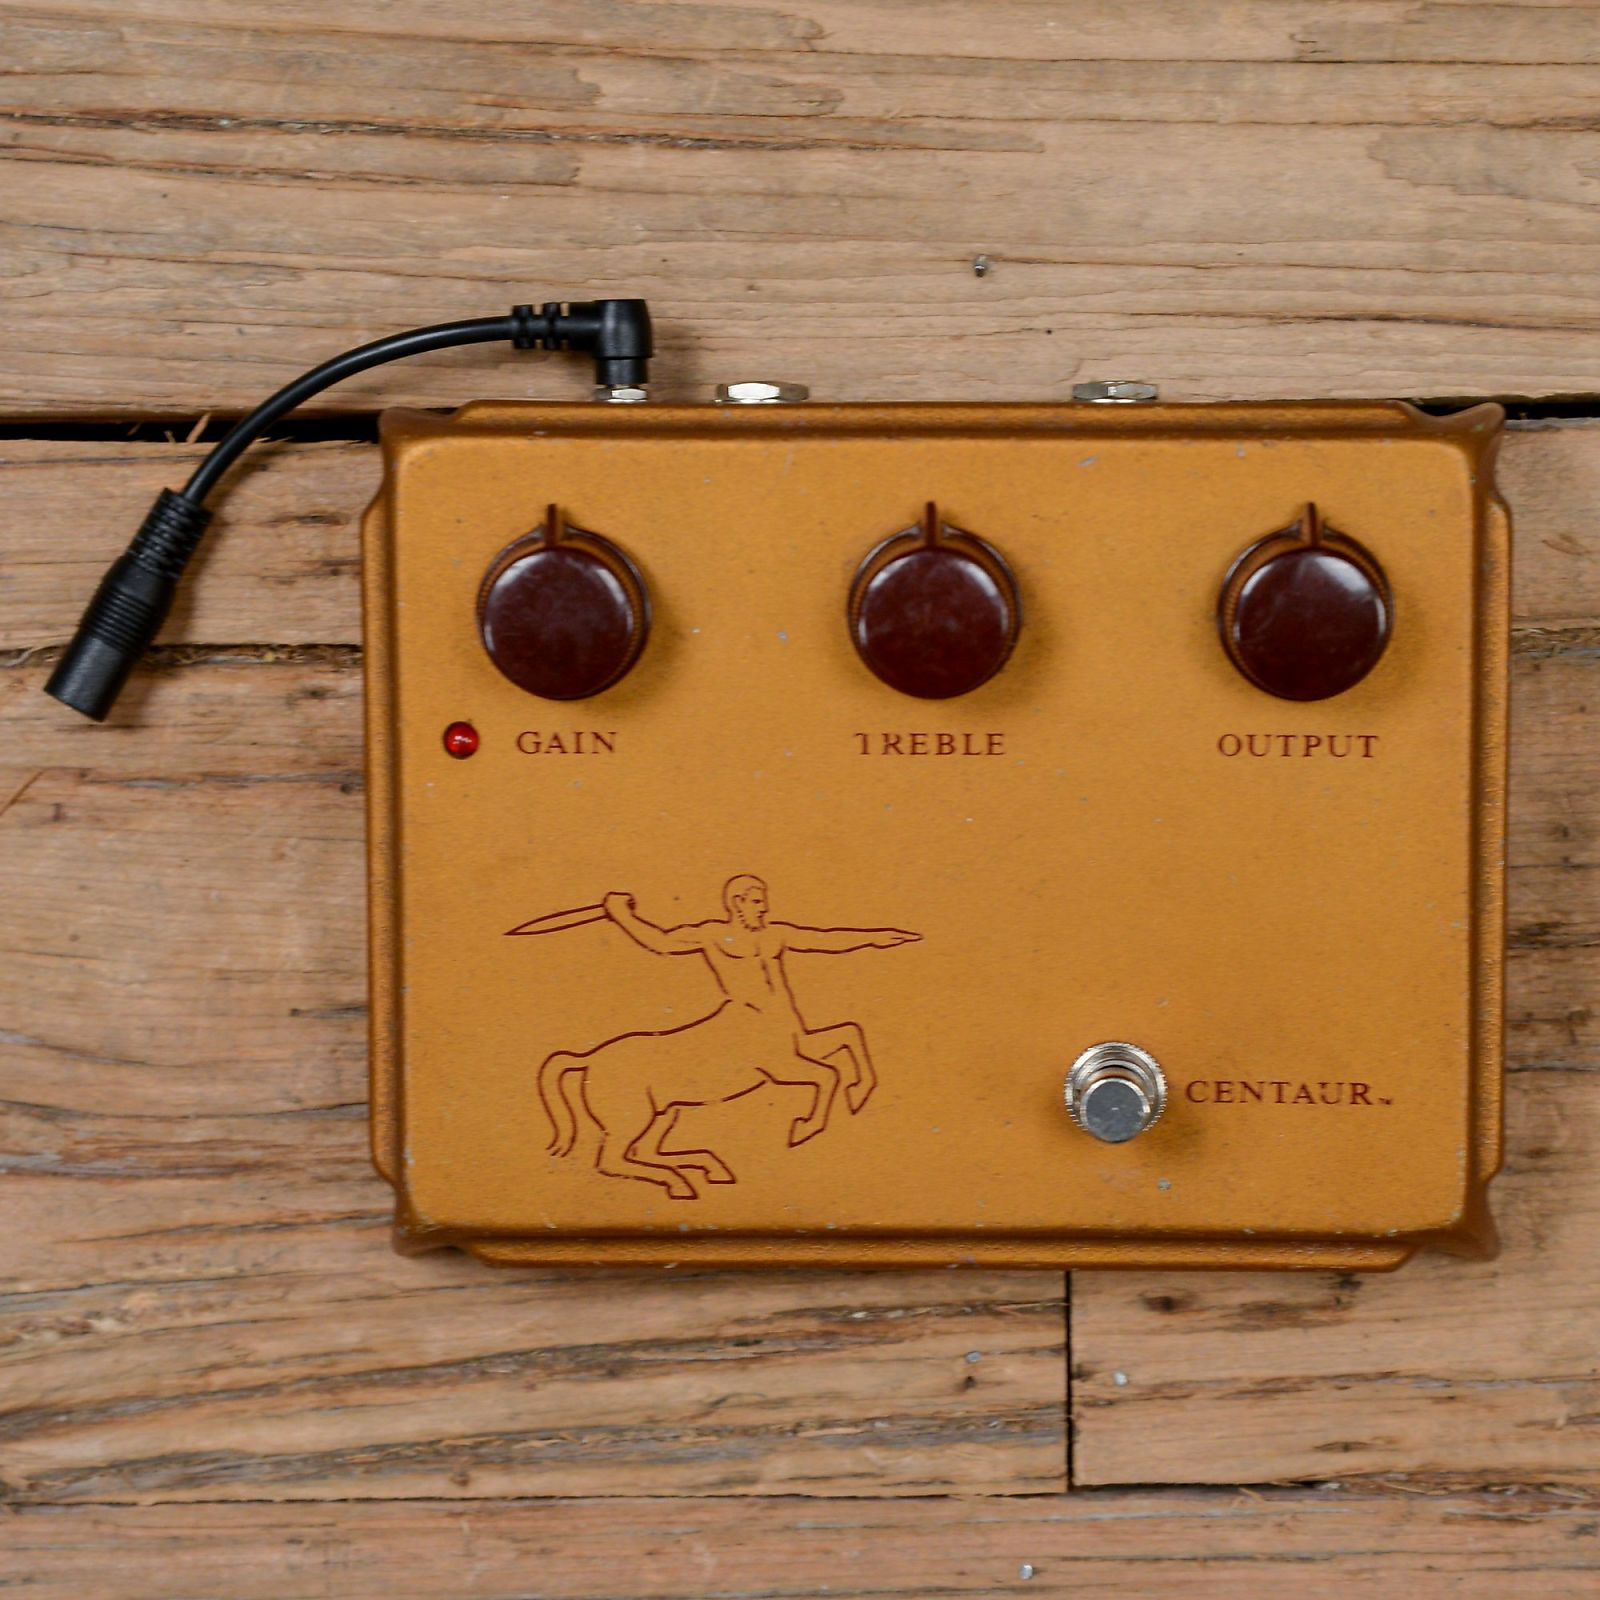
\includegraphics[height=2.5in]{../Paper/Figures/KlonCentaur.jpg}
    \end{figure}
\end{frame}

\begin{frame}{Virtual Analog Modelling}
    Creating a digital emulation of a classic analog audio effects.
    \vspace{1ex}
    \begin{itemize}
        \itemsep0.5em
        \item Provide access to effects that are old or rare.
        \item Lower cost.
        \item Convenience.
        \item Improved understanding.
    \end{itemize}
\end{frame}

\begin{frame}{``White-Box'' Modelling}
    Modelling a circuit through mathematical simulations of
    the physical interactions of the component parts.
    \vspace{1ex}
    \begin{itemize}
        \itemsep0em
        \item Nodal Analysis
        \item Modified Nodal Analysis (MNA)
        \item State-Space Formulation
        \item Wave Digital Filters (WDF)
        \item Port-Hamiltonian Formulation
    \end{itemize}
\end{frame}

\begin{frame}{``White-Box'' Modelling}
    \begin{columns}
        \begin{column}{0.5\linewidth}
            \hspace{-1ex}
            Advantages:
            \vspace{1ex}
            \begin{itemize}
                \itemsep0.5em
                \item Accurate modelling of circuit behaviour (even in extreme situations)
                \item Accurate modelling of control parameters
                \item Improved understanding of the modelled effect
            \end{itemize}
        \end{column}
        \begin{column}{0.5\linewidth}
            \hspace{-1ex}
            Disadvantages:
            \vspace{1ex}
            \begin{itemize}
                \itemsep0.5em
                \item Often computationally expensive (especially for real-time use) 
                \item Requires knowledge of DSP, as well as physics, circuit theory, etc.
            \end{itemize}
        \end{column}
    \end{columns}
\end{frame}

\begin{frame}{``Black-Box'' Modelling}
    Modelling a circuit by taking measurements, and designing a system
    to give a perceptually equivalent output.
    \vspace{1ex}
    \begin{itemize}
        \itemsep0em
        \item Convolution with Impulse Response (for linear systems)
        \item Volterra Series
        \item Weiner-Hammerstein Method
        \item Neural Networks
    \end{itemize}
\end{frame}

\begin{frame}{``Black-Box'' Modelling}
    \begin{columns}
        \begin{column}{0.5\linewidth}
            \hspace{-1ex}
            Advantages:
            \vspace{1ex}
            \begin{itemize}
                \itemsep0.5em
                \item Better for capturing ``unique'' behaviour
                \item Computationally cheaper
                \item Only requires background knowledge of DSP
            \end{itemize}
        \end{column}
        \begin{column}{0.5\linewidth}
            \hspace{-1ex}
            Disadvantages:
            \vspace{1ex}
            \begin{itemize}
                \itemsep0.5em
                \item Difficult to include control parameters
                \item Minimal understanding of the effect being modelled
            \end{itemize}
        \end{column}
    \end{columns}
\end{frame}

\begin{frame}{Different Platforms}
    \begin{columns}
        \begin{column}{0.5\linewidth}
            \hspace{-1ex}
            Desktop Audio Plugin:
            \vspace{1ex}
            \begin{itemize}
                \itemsep0.5em
                \item Consumer-grade CPU
                \item Plenty of memory
                \item Have to share resources with other plugins
            \end{itemize}
        \end{column}
        \begin{column}{0.5\linewidth}
            \hspace{-1ex}
            Embedded Device:
            \vspace{1ex}
            \begin{itemize}
                \itemsep0.5em
                \item Depends on the device (pedal, Eurorack module, multi-effects processor)
                \item More powerful processors are more expensive
                \item Limited memory
                \item (Usually) don't have to share resources
            \end{itemize}
        \end{column}
    \end{columns}
\end{frame}

\begin{frame}{Research Goals}
    \begin{itemize}
        \item Model sub-circuits from the Klon Centaur using different modelling methods:
        \begin{itemize}
            \itemsep0em
            \item Nodal Analysis
            \item Wave Digital Filters
            \item Neural Networks
        \end{itemize}
        \item Create desktop and embedded implementations of the modelled effect
        \item Compare the advantages/disadvantages of each method
    \end{itemize}
\end{frame}

\begin{frame}{Outline}
    \begin{itemize}
        \item Traditional Circuit Modelling
        \begin{itemize}
            \itemsep0em
            \item Nodal Analysis (Tone Stage sub-circuit)
            \item Wave Digital Filters (FF-1 sub-circuit)
        \end{itemize}
        \item Neural Network Circuit Modelling
        \begin{itemize}
            \itemsep0em
            \item Recurrent Neural Network (Gain Stage sub-circuit)
        \end{itemize}
        \item Desktop and embedded implementations
        \item Comparisons and Results
    \end{itemize}
\end{frame}
